\documentclass[11pt]{article}
%	options include 12pt or 11pt or 10pt
%	classes include article, report, book, letter, thesis

\usepackage{amsmath}
\usepackage{array}
\setlength\extrarowheight{2pt}
\usepackage{graphicx}
\graphicspath{ {/home/shanedrafahl/coms331/hw0} }

\title{HW0}
\author{Shane Drafahl}
\date{23 August,2017}

\begin{document}
\maketitle

\fbox{\parbox{\dimexpr\linewidth-2\fboxsep-2\fboxrule\relax}{
 This is an inline equation $x + y = 3$  \\
 This is a displayed equation: \\
 \large \centerline{ $ x + \dfrac{y}{z - \sqrt{3}} = 2 $} \\
 This is how you define a piece-wise linear function: \\
 $$
f(x) = \left\{
        \begin{array}{ll}
        3x + 2 & $if x $<$ 0$ \\
        7x + 2 & $if x $ \geq $ 0 and x $<$ 10$ \\
        5x + 22 & $otherwise.$ \\
        \end{array}
    \right.
$$ \\

This is a matrix:
    \begin{center}
    \begin{tabular}{ |l|l|l|l| }

    \hline
    9 & 9 & 9 & 9 \\ [0.5ex]
    \hline
    6 & 6 & 6 &  \\ [0.5ex]
    \hline
    3 &  & 3 & 3 \\ [0.5ex]
    \hline
    \end{tabular}
    \end{center}

    This is a figure incorporated in a LaTeX file \\
    \\
    \centerline{ 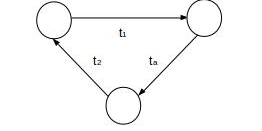
\includegraphics{graph.jpg} }
}}

$\newline$
2. Show that N (natural numbers) and Z (integer numbers) are equinumerous.
$\newline$
To show that the set of natural numbers and integer numbers are equinumerous
we have to show the cardinality of N and Z are the same. If there is a function
f: N $\rightarrow$ Z that is bijective then the cardinalities of sets N and Z would
be the same.
\newline

Suppose we have a function where $x \in N$ and $f(x) \in Z$

$$
f(x) = \left\{
        \begin{array}{ll}
        0 & $if x equals 0$ \\
        \frac{x}{2} * -1 & $if x mod 2 = 0$ \\
        \frac{(x - 1)}{2} + 1 & $otherwise.$ \\
        \end{array}
    \right.
$$ \\

If f is onto then $\forall_{y} \in $ Z $ \exists_{x} \in N $ where $ f(x) = y $.
Using existential instantiation and universal instantiation either
$\frac{x}{2} * -1 = y$ or $\frac{(x - 1)}{2} + 1 = y$. If $ \frac{x}{2} * -1 = y $.
For $\frac{x}{2} * -1 = y$ is equal to x = -2y and $\frac{(x - 1)}{2} + 1 = y$ equals
2y - 1 = x. If y is negative then for -2y = x, x will equal a natural number. If y is positive
then 2y - 1 = x, x will equal a natural number because it cannot be negative and y cant be 0 because
x will be 0 as well. So therefore for all values of y a natural number of x can be reached so therefor
function f is onto.
$\newline$
Using proof by contradiction assume f is not one to one so $\exists_{x}\exists_{y}(f(x) = f(y)
\rightarrow x \neq y \land x, y \in N \land x, y)$. If x is odd and y is even or vice versa then
$\frac{y}{2} * -1 = $\frac{(x - 1)}{2} + 1. This can be reduced to y = -x - 1. This is a contradiction
because since x and y are natural numbers they cannot be negative so $ 0 > -x - 1 $ and $ y > 0 $ so therefore
they cannot be equal. If x and y are both even then \frac{y}{-2} = \frac{x}{-2} which reduces to
x = y which is a contradiction because x and y cannot equal each other. If x and y are both odd then
$ \frac{(y - 1)}{2} + 1 $ = $ \frac{(x - 1)}{2} + 1 $ which reduces down to x = y and for the same
reason is a contradiction because x and y equal each other.
$\newline$
therefore the function f is one to one and onto so it is bijunction and therefore natural
numbers have the same cardinality as integers and are are equinumerous.




\end{document}
